\chapter{Nuclear Models Solutions}
\begin{abox}
	Practice Set-1
\end{abox}
\begin{enumerate}
	\item  The root-mean-square (r.m.s) energy of a nucleon in a nucleus of atomic number $A$ in its ground state varies as:
	\begin{tasks}(4)
		\task[\textbf{a.}]$A^{4 / 3}$
		\task[\textbf{b.}]$A^{1 / 3}$
		\task[\textbf{c.}]$A^{-1 / 3}$
		\task[\textbf{d.}]$A^{-2 / 3}$ 
	\end{tasks}
	\begin{answer}
		So the correct answer is \textbf{Option(c)}
	\end{answer}
	\item  Let $E_S$ denotes the contribution of the surface energy per nucleon in the liquid drop model. The ratio $E_S\left({ }_{13}^{27} \mathrm{Al}\right): E_S\left({ }_{30}^{64} \mathrm{Zn}\right)$ is
	{\exyear{NET/JRF (JUNE-2016)}}
	\begin{tasks}(4)
		\task[\textbf{a.}]$2: 3$
		\task[\textbf{b.}]$4: 3$
		\task[\textbf{c.}]$5: 3$
		\task[\textbf{d.}]$3: 2$ 
	\end{tasks}
	\begin{answer}
		\begin{align*}
		E_S=\frac{B}{A}=\frac{A^{\frac{2}{3}}}{A} \propto A^{-\frac{1}{3}} \Rightarrow \frac{E_S(A l)}{E_S\left(Z_n\right)}=\frac{(27)^{-\frac{1}{3}}}{(64)^{-\frac{1}{3}}}=\frac{(64)^{\frac{1}{3}}}{(27)^{\frac{1}{3}}}=\frac{4}{3}
		\end{align*}
		So the correct answer is \textbf{Option(b)}
	\end{answer}
	\item  The binding energy of a light nucleus $(Z, A)$ in $\mathrm{MeV}$ is given by the approximate formula
	$$
	B(A, Z) \approx 16 A-20 A^{2 / 3}-\frac{3}{4} Z^2 A^{-1 / 3}+30 \frac{(N-Z)^2}{A}
	$$
	where $N=A-Z$ is the neutron number. The value of $Z$ of the most stable isobar for a $\operatorname{given} A$ is
	{\exyear{ 	NET/JRF (JUNE-2013)}}
	\begin{tasks}(2)
		\task[\textbf{a.}] $\frac{A}{2}\left(1-\frac{A^{2 / 3}}{160}\right)^{-1}$
		\task[\textbf{b.}]$\frac{A}{2}$
		\task[\textbf{c.}]$\frac{A}{2}\left(1-\frac{A^{2 / 3}}{120}\right)^{-1}$
		\task[\textbf{d.}] $\frac{A}{2}\left(1+\frac{A^{4 / 3}}{64}\right)^{-1}$
	\end{tasks}
	\begin{answer}
		\begin{align*}
		\left.\frac{\partial B}{\partial Z}\right|_{Z=Z^{\prime}}=0 \Rightarrow Z^{\prime}=\frac{A}{2}\left(1-\frac{A^{2 / 3}}{160}\right)^{-1}
		\end{align*}
		So the correct answer is \textbf{Option(a)}
	\end{answer}
	\item  If the binding energy $B$ of a nucleus (mass number $A$ and charge $Z$ ) is given by
	$$
	B=a_V A-a_S A^{2 / 3}-a_{s y m} \frac{(2 Z-A)^2}{A}+\frac{a_c Z^2}{A^{1 / 3}}
	$$
	where $a_V=16 \mathrm{MeV}, a_S=16 \mathrm{MeV}, a_{s y m}=24 \mathrm{MeV}$ and $a_C=0.75 \mathrm{MeV}$, then for the most stable isobar for a nucleus with $A=216$ is
	{\exyear{ 	NET/JRF (DEC-2014)}}
	\begin{tasks}(4)
		\task[\textbf{a.}]68
		\task[\textbf{b.}]72
		\task[\textbf{c.}]84
		\task[\textbf{d.}]92
	\end{tasks}
	\begin{answer}
		\begin{align*}
		&\text{ For the most stable isobar for a nucleus }\frac{d B}{d Z}=0 \Rightarrow-a_{s y m} \frac{2(2 Z-A) \times 2}{A}+\frac{2 a_C Z}{A^{1 / 3}}=0\\
		&\Rightarrow 24 \frac{2(2 Z-216) \times 2}{216}+0.75 \frac{2 Z}{(216)^{1 / 3}}=0 \Rightarrow \frac{4(2 Z-216)}{9}+\frac{3}{4} \frac{2 Z}{6}=0 \\
		&\Rightarrow \frac{4(2 Z-216)}{9}+\frac{Z}{4}=0 \Rightarrow 16(2 Z-216)+9 Z=0 \Rightarrow 41 Z=216 \times 16 \Rightarrow Z=82.3
		\end{align*}
		So the correct answer is \textbf{Option(c)}
	\end{answer}
	\item  Of the nuclei of mass number $A=125$, the binding energy calculated from the liquid drop model (given that the coefficients for the Coulomb and the asymmetry energy are $a_c=0.7 \mathrm{MeV}$ and $a_{s y m}=22.5 \mathrm{MeV}$ respectively) is a maximum for
	{\exyear{ 	NET/JRF (DEC-2015)}}
	\begin{tasks}(4)
		\task[\textbf{a.}]${ }_{54}^{125} \mathrm{Xe}$
		\task[\textbf{b.}]${ }_{53}^{124} I$
		\task[\textbf{c.}]${ }_{52}^{125} \mathrm{Te}$
		\task[\textbf{d.}]  ${ }_{51}^{125} \mathrm{Sb}$
	\end{tasks}
	\begin{answer}
		\begin{align*}
		Z_0&=\frac{4 a_a+a_c A^{-1 / 3}}{2 a_c A^{-1 / 3}+8 a_a A^{-1}}=\frac{4 a_a A+a_c A^{2 / 3}}{8 a_a+2 a_c A^{2 / 3}} \Rightarrow Z_0=\frac{4 \times 22.5 \times 125+0.7\left(5^3\right)^{2 / 3}}{8 \times 22.5+2 \times 0.7\left(5^3\right)^{2 / 3}} \\
		\Rightarrow Z_0&=\frac{11250+17.5}{180+35}=\frac{11267.5}{215}=52.4 \Rightarrow Z_0 \approx 52
		\end{align*}
		So the correct answer is \textbf{Option(c)}
	\end{answer}
	\item  The Bethe-Weizsacker formula for the binding energy (in $\mathrm{MeV}$ ) of a nucleus of atomic number $Z$ and mass number $A$ is
	$$
	15.8 A-18.3 A^{2 / 3}-0.714 \frac{Z(Z-1)}{A^{1 / 3}}-23.2 \frac{(A-2 Z)^2}{A}
	$$
	The ratio $Z / A$ for the most stable isobar of a $A=64$ nucleus, is nearest to
	\begin{tasks}(4)
		\task[\textbf{a.}]$0.30$
		\task[\textbf{b.}] $0.35$
		\task[\textbf{c.}]$0.45$
		\task[\textbf{d.}]$0.50$ 
	\end{tasks}
	\begin{answer}
		\begin{align*}
		Z_0&=\frac{A}{2+\frac{a_c}{2 a_a} A^{2 / 3}} \Rightarrow \frac{Z_0}{A}=\frac{1}{2+\frac{a_c}{2 a_a} A^{2 / 3}}\\
		\text{ given }a_c&=0.714\text{ and }a_a=23.2\\
		\therefore \quad\frac{Z_0}{A}&=\frac{1}{2+\frac{0.714}{2 \times 23.2} A^{2 / 3}}=\frac{1}{2+0.015 A^{2 / 3}}=\frac{1}{2+0.015(64)^{2 / 3}}=0.45
		\end{align*}
		So the correct answer is \textbf{Option (c)}
	\end{answer}
	\item  Let us approximate the nuclear potential in the shell model by a three dimensional isotropic harmonic oscillator. Since the lowest two energy levels have angular momenta $l=0$ and $l=1$ respectively, which of the following two nuclei have magic numbers of protons and neutrons?
	{\exyear{ 	NET/JRF (JUNE-2015)}}
	\begin{tasks}(2)
		\task[\textbf{a.}]${ }_2^4 \mathrm{He}$ and ${ }_8^{16} \mathrm{O}$
		\task[\textbf{b.}]${ }_1^2 D$ and ${ }_4^8 B e$
		\task[\textbf{c.}]${ }_2^4 \mathrm{He}$ and ${ }_4^8 \mathrm{Be}$
		\task[\textbf{d.}] ${ }_2^4 \mathrm{He}$ and ${ }_6^{12} \mathrm{C}$
	\end{tasks}
	\begin{answer}
		\begin{align*}
		&{ }_2 H e^4\text{ has }Z=2, N=2\\
		&\text{	and }{ }_8 O^{16}\text{ has $Z=8, N=8$ magic numbers $(2,8,20,28,50,82,126)$}
		\end{align*}
		So the correct answer is \textbf{Option (a)}
	\end{answer}
	\item  According to the shell model the spin and parity of the two nuclei ${ }_{51}^{125} \mathrm{Sb}$ and ${ }_{38}^{89} \mathrm{Sr}$ are, respectively,
	{\exyear{ 	NET/JRF (DEC-2011)}}
	\begin{tasks}(2)
		\task[\textbf{a.}]$\left(\frac{5}{2}\right)^{+}$and $\left(\frac{5}{2}\right)^{+}$
		\task[\textbf{b.}]$\left(\frac{5}{2}\right)^{+}$and $\left(\frac{7}{2}\right)^{+}$
		\task[\textbf{c.}]$\left(\frac{7}{2}\right)^{+}$and $\left(\frac{5}{2}\right)^{+}$
		\task[\textbf{d.}] $\left(\frac{7}{2}\right)^{+}$and $\left(\frac{7}{2}\right)^{+}$
	\end{tasks}
	\begin{answer}
		\begin{align*}
		{ }_{51}^{125} \mathrm{Sb} ; Z&=51 \text { and } N=74\\
		Z&=51 \\
		&\left(s_{1 / 2}\right)^2\left(p_{3 / 2}\right)^4\left(p_{1 / 2}\right)^2\left(d_{5 / 2}\right)^6\left(s_{1 / 2}\right)^2\left(d_{3 / 2}\right)^4\left(f_{7 / 2}\right)^8\left(p_{3 / 2}\right)^4\left(f_{5 / 2}\right)^6\left(p_{1 / 2}\right)^2\left(g_{9 / 2}\right)^{10}\left(g_{7 / 2}\right)^1 \\
		\Rightarrow j&=\frac{7}{2} \text { and } l=4 \text {. Thus spin and parity }=\left(\frac{7}{2}\right)^{+} \\
		{ }_{38}^{89} S r ; Z&=38 \text { and } N=51 \\
		N&=51 \text { : } \\
		&\left(s_{1 / 2}\right)^2\left(p_{3 / 2}\right)^4\left(p_{1 / 2}\right)^2\left(d_{5 / 2}\right)^6\left(s_{1 / 2}\right)^2\left(d_{3 / 2}\right)^4\left(f_{7 / 2}\right)^8\left(p_{3 / 2}\right)^4\left(f_{5 / 2}\right)^6\left(p_{1 / 2}\right)^2\left(g_{9 / 2}\right)^{10}\left(g_{7 / 2}\right)^1 \\
		\Rightarrow j&=\frac{7}{2} \text { and } l=4 \text {. Thus spin and parity }=\left(\frac{7}{2}\right)^{+}
		\end{align*}
		So the correct answer is \textbf{Option (d)}
	\end{answer}
	\item  According to the shell model, the total angular momentum (in units of $\hbar$ ) and the parity of the ground state of the ${ }_3^7 L i$ nucleus is
	{\exyear{ 	NET/JRF (DEC-2013)}}
	\begin{tasks}(2)
		\task[\textbf{a.}]$\frac{3}{2}$ with negative parity
		\task[\textbf{b.}]$\frac{3}{2}$ with positive parity
		\task[\textbf{c.}]$\frac{1}{2}$ with positive parity
		\task[\textbf{d.}] $\frac{7}{2}$ with negative parity
	\end{tasks}
	\begin{answer}
		\begin{align*}
		Z&=3, N=4\\
		\text{For odd }Z&=3 ;\left(s_{1 / 2}^2\right)\left(p_{3 / 2}^1\right) \Rightarrow j=3 / 2, l=1\text{ and parity $=(-1)^1=-1$.}
		\end{align*}
		So the correct answer is \textbf{Option (a)}
	\end{answer}
	\item  According to the shell model, the nuclear magnetic moment of the ${ }_{13}^{27} \mathrm{Al}$ nucleus is (Given that for a proton $g_l=1, g_s=5.586$, and for a neutron $g_l=0, g_s=-3.826$ )
	{\exyear{ 	NET/JRF (JUNE-2016)}}
	\begin{tasks}(4)
		\task[\textbf{a.}] $-1.913 \mu_N$
		\task[\textbf{b.}] $14.414 \mu_N$
		\task[\textbf{c.}]$4.793 \mu_N$
		\task[\textbf{d.}]0 
	\end{tasks}
	\begin{answer}
		\begin{align*}
		&\text{ ${ }_{13} A l^{27}: Z=13, N=14$ for $Z=13, S_{1 / 2}^2, P_{3 / 2}^4, P_{1 / 2}^2, d_{5 / 2}^5 \Rightarrow j=\frac{5}{2}, l=2$}\\
		&\text{Magnetic moment, $\mu=\frac{1}{2}\left[2 j-1+g_S\right] \mu_N=\frac{1}{2}\left[2 \times \frac{5}{2}-1+5.586\right] \mu_N \Rightarrow \mu=4.793 \mu_N$}
		\end{align*}
		So the correct answer is \textbf{Option (c)}
	\end{answer}
	\item  The spin-parity assignments for the ground and first excited states of the isotope ${ }_{28}^{57} \mathrm{Ni}$, in the single particle shell model, are
	{\exyear{ 	NET/JRF (DEC-2017)}}
	\begin{tasks}(2)
		\task[\textbf{a.}]$\left(\frac{1}{2}\right)^{-}$and $\left(\frac{3}{2}\right)^{-}$
		\task[\textbf{b.}] $\left(\frac{5}{2}\right)^{+}$and $\left(\frac{7}{2}\right)^{+}$
		\task[\textbf{c.}]$\left(\frac{3}{2}\right)^{+}$and $\left(\frac{5}{2}\right)^{+}$
		\task[\textbf{d.}] $\left(\frac{3}{2}\right)^{-}$and $\left(\frac{5}{2}\right)^{-}$
	\end{tasks}
	\begin{answer}
		\begin{align*}
		&\text{Spin parity for ${ }_{28} \mathrm{Ni}^{57}$ for ground state and first excited   state}\\
		&\text{ For ${ }_{28} N i^{57}: \quad P=28, N=29 \rightarrow$ will decide the $j^P$ }\\
		&\text{ So, for $N=29$, ground state configuration,}\\
		&\text{$1 s_{1 / 2}^2 1 p_{3 / 2}^4 1 p_{1 / 2}^2 1 d_{5 / 2}^6 2 s_{1 / 2}^2 1 d_{3 / 2}^4 1 f_{7 / 2}^8 2 p_{3 / 2}^1$}\\
		&\text{So, $j=\frac{3}{2}, l=1$}\\
		&\text{Spin parity for ground state of ${ }_{28} \mathrm{Ni}^{57} \rightarrow\left(\frac{3}{2}\right)^{-}$}\\
		&\text{For first excited state,}\\
		&1 s_{1 / 2}^2 1 p_{3 / 2}^4 1 p_{1 / 2}^2 1 d_{5 / 2}^6 2 s_{1 / 2}^2 1 d_{3 / 2}^4 1 f_{7 / 2}^8 2 p_{3 / 2}^1 \rightarrow 1 f_{5 / 2}\\
		&\text{$P=\frac{5}{2}, l=3 \Rightarrow$ spin parity $\rightarrow\left(\frac{5}{2}\right)^{-}$}
		\end{align*}
		So the correct answer is \textbf{Option (d)}
	\end{answer}
	\item  The first excited state of the rotational spectrum of the nucleus ${ }_{92}^{238} U$ has an energy $45 \mathrm{keV}$ above the ground state. The energy of the second excited state (in $\mathrm{keV}$ ) is
	{\exyear{	NET/JRF (DEC-2017)}}
	\begin{tasks}(4)
		\task[\textbf{a.}]150
		\task[\textbf{b.}]120
		\task[\textbf{c.}]90
		\task[\textbf{d.}] 60
	\end{tasks}
	\begin{answer}
		\begin{align*}
		\text{As per the }&\text{shell model (Collective Model)}\\
		\text{	Rotational}&\text{ Energies,}\\
		E_r=\frac{\hbar^2}{2 I} J(J+1), I \rightarrow&\text{ is moment of inertia where only even value of $J$ are allowed }\\
		\text{	i.e., }J&=0^{+}, 2^{+}, 4^{+}, 6^{+}, \ldots \ldots.\\
		\text{Now, for ground state }J&=0^{+}, E=0 \mathrm{keV}\\
		\text{For first excited state, }J&=2^{+}, E=45 \mathrm{keV}\text{ (given)}\\
		\text{So, }45 \mathrm{keV}&=\frac{\hbar^2}{2 I} \cdot 2 \cdot 3\text{ or,} \frac{\hbar^2}{2 I}=\frac{45}{6} \mathrm{keV}..(i)\\
		\text{Now, for }&\text{second excited state, }J=4^{+}\\
		E_2&=\frac{\hbar^2}{2 I} \cdot 4 \cdot 5\text{ (put value of $\frac{\hbar^2}{2 I}$ from (i))}\\
		\text{	or, }E_2&=\frac{45}{6} \times 20=\frac{900}{6}=150 \mathrm{keV}.
		\end{align*}
		So the correct answer is \textbf{150}
	\end{answer}
	\item  The low lying energy levels due to the vibrational excitations of an even-even nucleus are shown in the figure below,\\
	The spin-parity $j^p$ of the level $E_1$ is
	{\exyear{ 	NET/JRF (DEC-2018)}}
	\begin{tasks}(4)
		\task[\textbf{a.}]$1^{+}$
		\task[\textbf{b.}]$1^{-}$
		\task[\textbf{c.}]$2^{-}$
		\task[\textbf{d.}]$2^{+}$ 
	\end{tasks}
	\begin{answer}
		Quadrupole oscillations are the lowest order nuclear vibrational mode. The quanta of vibrational energy are called phonons. A quadrupole phonon carries 2 units of angular momentum. Therefore, the parity is $P=(-1)^2=+v e$\\
		Also, the even-even ground state is $O^{+}$. The 1 phonon excited state is $2^{+}$. The 2 phonons excited states are $0^{+}, 2^{+}, 4^{+}$. Thus correct option is (a)\\\\
		$\left.\begin{array}{ll}1.35\text{ -------}& 0^{+} \\ 1.25 \text{ -------}& 2^{+} \\ 1.17 \text{ -------}& 4^{+}\end{array}\right\} 2$-phonons\\
		$0.56\text{ -------}2^{+}: 1$-phonon\\
		0 $\text{ -------}0^{+}$:Ground state\\
		meV\\
		So the correct answer is \textbf{Option (d)}
	\end{answer}
	\item  An excited state of a ${ }_4^8 B e$ nucleus decays into two $\alpha$-particles which are in a $\quad$ spinparity $0^{+}$state. If the mean life-time of this decay is $10^{-22} \mathrm{~s}$, the spin-parity of the excited state of the nucleus is
	\begin{tasks}(4)
		\task[\textbf{a.}]$2^{+}$
		\task[\textbf{b.}]$3^{+}$
		\task[\textbf{c.}]$0^{-}$
		\task[\textbf{d.}]$4^{-}$ 
	\end{tasks}
	\begin{answer}
		The parity angular momentum selection rule in $\alpha$-decay says that, if the initial and final particles are same, the $I_\alpha$ must be even; if the parties are different, then $I_\alpha$ must be odd.\\	The ground state is $0^{+}$thus spin-parity of excited state must be $2^{+}$. Thus correct option is (a)\\\\
		So the correct answer is \textbf{Option (a)}
	\end{answer}
\end{enumerate}
 \colorlet{ocre1}{ocre!70!}
\colorlet{ocrel}{ocre!30!}
\setlength\arrayrulewidth{1pt}
\begin{table}[H]
	\centering
	\arrayrulecolor{ocre}
	\begin{tabular}{|p{1.5cm}|p{1.5cm}||p{1.5cm}|p{1.5cm}|}
		\hline
		\multicolumn{4}{|c|}{\textbf{Answer key}}\\\hline\hline
		\rowcolor{ocrel}Q.No.&Answer&Q.No.&Answer\\\hline
		1&\textbf{c} &2&\textbf{b}\\\hline 
		3&\textbf{a} &4&\textbf{c} \\\hline
		5&\textbf{c} &6&\textbf{c} \\\hline
		7&\textbf{a}&8&\textbf{d}\\\hline
		9&\textbf{a}&10&\textbf{c}\\\hline
		11&\textbf{d} &12&\textbf{}\\\hline
		13&\textbf{d}&14&\textbf{a}\\\hline
		15&\textbf{}& &\\\hline
		
	\end{tabular}
\end{table}



\newpage
\begin{abox}
	Practice Set-2
\end{abox}
\begin{enumerate}
	\item The semi-empirical mass formula for the binding energy of nucleus contains a surface correction term. This term depends on the mass number $A$ of the nucleus as
	{\exyear{	GATE-2011}}
	\begin{tasks}(4)
		\task[\textbf{a.}]$A^{-1 / 3}$
		\task[\textbf{b.}]$A^{1 / 3}$
		\task[\textbf{c.}]$A^{2 / 3}$
		\task[\textbf{d.}] $A$
	\end{tasks}
	\begin{answer}
		So the correct answer is \textbf{Option (c)}
	\end{answer}
	\item  The nuclear spin and parity of ${ }_{20}^{40} \mathrm{Ca}$ in its ground state is
	{\exyear{ 	GATE-2019}}
	\begin{tasks}(4)
		\task[\textbf{a.}]$0^{+}$
		\task[\textbf{b.}]$0^{-}$
		\task[\textbf{c.}]$1^{+}$
		\task[\textbf{d.}] $1^{-}$
	\end{tasks}
	\begin{answer}
		\begin{align*}
		&\text{ ${ }_{20}^{40} \mathrm{Ca}$ is an even-even nuclei, therefore $I=0, P=+v e$}\\
		&\therefore \quad \text { Spin-parity }=0^{+}
		\end{align*}
		So the correct answer is \textbf{Option (a)}
	\end{answer}
	\item  In the nuclear shell model, the spin parity of ${ }_7^{15} N$ is given by
	{\exyear{	GATE-2010}}
	\begin{tasks}(4)
		\task[\textbf{a.}]$\frac{1^{-}}{2}$
		\task[\textbf{b.}]$\frac{1^{+}}{2}$
		\task[\textbf{c.}]$\frac{3^{-}}{2}$
		\task[\textbf{d.}]$\frac{3^{+}}{2}$
	\end{tasks}
	\begin{answer}
		\begin{align*}
		&\text{$Z=7 ;\left(s_{1 / 2}\right)^2\left(p_{3 / 2}\right)^4\left(p_{1 / 2}\right)^1$ and $N=8$}\\
		&l=1, J=\frac{1}{2} \Rightarrow \text { parity }=(-1)^1=-1, \quad \text { spin }-\text { parity }=\left(\frac{1}{2}\right)^{-}
		\end{align*}
		So the correct answer is \textbf{Option (a)}
	\end{answer}
	\item  According to the nuclear shell model, the respective ground state spin-parity values of ${ }_8^{15} \mathrm{O}$ and ${ }_8^{17} \mathrm{O}$ nuclei are
	{\exyear{	GATE-2016}}
	\begin{tasks}(4)
		\task[\textbf{a.}]$\frac{1^{+}}{2}, \frac{1^{-}}{2}$
		\task[\textbf{b.}] $\frac{1}{2}^{-}, \frac{5^{+}}{2}$
		\task[\textbf{c.}]$\frac{3^{-}}{2}, \frac{5^{+}}{2}$
		\task[\textbf{d.}] $\frac{3^{-}}{2}, \frac{1^{-}}{2}$
	\end{tasks}
	\begin{answer}
		\begin{align*}
		&\text{ ${ }_8^{15} O ; Z=8$ and $N=7 ; \quad N=7:\left(s_{1 / 2}\right)^2\left(p_{3 / 2}\right)^4\left(p_{1 / 2}\right)^1$ }\\
		&\text{$\Rightarrow j=\frac{1}{2}$ and $l=1$. Thus spin and parity $=\left(\frac{1}{2}\right)^{-}$ }\\
		&\text{${ }_8^{17} O ; Z=8$ and $N=9 ; \quad N=9:\left(s_{1 / 2}\right)^2\left(p_{3 / 2}\right)^4\left(p_{1 / 2}\right)^2\left(d_{5 / 2}\right)^1$} \\
		&\text{ $\Rightarrow j=\frac{5}{2}$ and $l=2$. Thus spin and parity $=\left(\frac{5}{2}\right)^{+}$}
		\end{align*}
		So the correct answer is \textbf{Option (b)}
	\end{answer}
	\item  $J^P$ for the ground state of the ${ }^{13} C_6$ nucleus is
	{\exyear{ 	GATE-2017}}
	\begin{tasks}(4)
		\task[\textbf{a.}]$1^{+}$
		\task[\textbf{b.}]$\frac{3^{-}}{2}$
		\task[\textbf{c.}]$\frac{3^{+}}{2}$
		\task[\textbf{d.}]$\frac{1^{-}}{2}$ 
	\end{tasks}
	\begin{answer}
		\begin{align*}
		&\text{ ${ }^{13} C_6: Z=6, N=7, N=7:\left(s_{1 / 2}\right)^2\left(p_{3 / 2}\right)^4\left(p_{1 / 2}\right)^1$ }\\
		&\text{$\Rightarrow j=\frac{1}{2}$ and $l=1$.}\\
		&\text{Thus, spin and parity $=\left(\frac{1}{2}\right)^{-}$}
		\end{align*}
		So the correct answer is \textbf{Option (d)}
	\end{answer}
	\item  According to the single particles nuclear shell model, the spin-parity of the ground state of ${ }_8^{17} \mathrm{O}$ is
	{\exyear{ GATE-2011}}
	\begin{tasks}(4)
		\task[\textbf{a.}]$\frac{1}{2}$
		\task[\textbf{b.}]$\frac{3}{2}$
		\task[\textbf{c.}]$\frac{3}{2}$
		\task[\textbf{d.}]$\frac{5^{+}}{2}$ 
	\end{tasks}
	\begin{answer}
		\begin{align*}
		&Z=8 \text { and } N=9 ;\left(s_{1 / 2}\right)^2\left(p_{3 / 2}\right)^4\left(p_{1 / 2}\right)^2\left(d_{5 / 2}\right)^1\\
		&l=2, J=\frac{5}{2} \Rightarrow \text { parity }=(-1)^2=+1, \text { spin }-\text { parity }=\left(\frac{5}{2}\right)^{+}
		\end{align*}
		So the correct answer is \textbf{Option (d)}
	\end{answer}
	\item The first three energy levels of ${ }^{228} T h_{90}$ are shown below
	\begin{figure}[H]
		\centering
		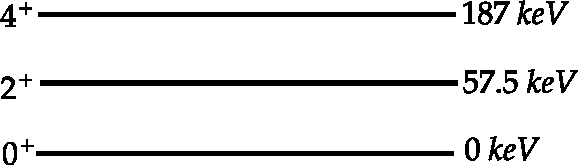
\includegraphics[height=1.8cm,width=6cm]{NM-1}
	\end{figure}
	The expected spin-parity and energy of the next level are given by
	{\exyear{ 	GATE-2010}}
	\begin{tasks}(2)
		\task[\textbf{a.}]$\left(6^{+} ; 400 \mathrm{keV}\right)$
		\task[\textbf{b.}]$\left(6^{+} ; 300 \mathrm{keV}\right)$
		\task[\textbf{c.}]$\left(2^{+} ; 400 \mathrm{keV}\right)$
		\task[\textbf{d.}] $\left(4^{+} ; 300 \mathrm{keV}\right)$
	\end{tasks}
	\begin{answer}
		\begin{align*}
		\frac{E_2}{E_1}=\frac{J_2\left(J_2+1\right)}{J_1\left(J_1+1\right)} \Rightarrow \frac{E_6}{E_4}=\frac{6(6+1)}{4(4+1)} \Rightarrow E_6=393 \mathrm{keV}
		\end{align*}
		So the correct answer is \textbf{Option (a)}
	\end{answer}
	\item  In the nuclear shell model, the potential is modeled as $V(r)=\frac{1}{2} m \omega^2 r^2-\lambda \vec{L} \cdot \vec{S}, \lambda>0$. The correct spin-parity and isospin assignments for the ground state of ${ }_6^{13} \mathrm{C}$ is
	{\exyear{	GATE-2015}}
	\begin{tasks}(2)
		\task[\textbf{a.}]$\frac{1^{-}}{2} ; \frac{-1}{2}$
		\task[\textbf{b.}]$\frac{1^{+}}{2} ; \frac{-1}{2}$
		\task[\textbf{c.}]$\frac{3^{+}}{2} ; \frac{1}{2}$
		\task[\textbf{d.}] $\frac{3^{-}}{2} ; \frac{-1}{2}$
	\end{tasks}
	\begin{answer}
		\begin{align*}
		&{ }^{13} C_6, \quad N=7, Z=6, \text { for } N=7 ; \quad\left(1 S_{\frac{1}{2}}\right)^2\left(1 P_{\frac{3}{2}}\right)^4\left(P_{\frac{1}{2}}\right)^1 \Rightarrow j=\frac{1}{2} \text { and } l=1\\
		&\text { Thus spin- parity is }\left(\frac{1}{2}\right)^{-} \text {. }
		\end{align*}
		So the correct answer is \textbf{Option (a)}
	\end{answer}
	\item  The total angular momentum $j$ of the ground state of the ${ }_8^{17} O$ nucleus is
	{\exyear{ 	GATE- 2020}}
	\begin{tasks}(4)
		\task[\textbf{a.}]$\frac{1}{2}$
		\task[\textbf{b.}]1
		\task[\textbf{c.}]$\frac{3}{2}$
		\task[\textbf{d.}]$\frac{5}{2}$ 
	\end{tasks}
	\begin{answer}
		\begin{align*}
		&\text{For ${ }_8^{17} O: z=8$ and $N=9$}\\
		&\text{For $N=9:\left(1 s_{1 / 2}\right)^2\left(1 p_{3 / 2}\right)^4\left(1 p_{1 / 2}\right)^2\left(1 d_{5 / 2}\right)^1$}\\
		&\text{The angular momentum is $I=\frac{5}{2}$}
		\end{align*}
		So the correct answer is \textbf{Option (d)}
	\end{answer}
	\item  For nucleus ${ }^{164} \mathrm{Er}$, a $J^\pi=2^{+}$state is at $90 \mathrm{keV}$. Assuming ${ }^{164} \mathrm{Er}$ to be a rigid rotor, the energy of its $4^{+}$state is -----------$\mathrm{keV}$ (up to one decimal place)
	{\exyear{	GATE-2018}}
	\begin{answer}$\left. \right. $
		\begin{figure}[H]
			\centering
			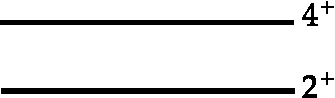
\includegraphics[height=1.2cm,width=4cm]{NM-2}
		\end{figure}
		\begin{align*}
		&\text{ $E_J=h c B J(J+1)$}\\
		&E_{2^{+}}=h c B 2(2+1) \text { and } E_{4^{+}}=h c B 4(4+1)\\
		&\text{Then, $\frac{E_{4^{+}}}{E_{2^{+}}}=\frac{20}{6} \Rightarrow E_{4^{+}}=\frac{20}{6} \times 90 \mathrm{keV}=300 \mathrm{keV}$}
		\end{align*}
	\end{answer}
\end{enumerate}
\colorlet{ocre1}{ocre!70!}
\colorlet{ocrel}{ocre!30!}
\setlength\arrayrulewidth{1pt}
\begin{table}[H]
	\centering
	\arrayrulecolor{ocre}
	\begin{tabular}{|p{1.5cm}|p{1.5cm}||p{1.5cm}|p{1.5cm}|}
		\hline
		\multicolumn{4}{|c|}{\textbf{Answer key}}\\\hline\hline
		\rowcolor{ocrel}Q.No.&Answer&Q.No.&Answer\\\hline
		1&\textbf{c} &2&\textbf{a}\\\hline 
		3&\textbf{a} &4&\textbf{b} \\\hline
		5&\textbf{d} &6&\textbf{d} \\\hline
		7&\textbf{a}&8&\textbf{a}\\\hline
		9&\textbf{d}&10&\textbf{300}\\\hline
		11&\textbf{} &12&\textbf{}\\\hline
		13&\textbf{}&14&\textbf{}\\\hline
		15&\textbf{}& &\\\hline
		
	\end{tabular}
\end{table}
